\documentclass[10pt,a4paper]{article}

% Packages
\usepackage[utf8]{inputenc}
\usepackage[T1]{fontenc}
\usepackage{lmodern}
\usepackage[margin=0.75in]{geometry}
\usepackage{graphicx}
\usepackage{booktabs}
\usepackage{amsmath}
\usepackage{hyperref}
\usepackage{xcolor}
\usepackage{pgfplots}
\usepackage{pgfplotstable}
\usepackage{siunitx}
\usepackage{caption}
\usepackage{subcaption}
\usepackage{float}
\usepackage{enumitem}
\usepackage{listings}
\usepackage{fancyhdr}
\usepackage{multirow}
\usepackage{multicol}

\pgfplotsset{compat=1.18}
\tolerance=1000
\emergencystretch=1em

\hypersetup{
    colorlinks=true,
    linkcolor=blue!60!black,
    citecolor=green!50!black,
    urlcolor=blue!70!black
}

\lstset{
    basicstyle=\ttfamily\small,
    backgroundcolor=\color{gray!10},
    frame=single,
    breaklines=true,
    columns=flexible
}

\pagestyle{fancy}
\fancyhf{}
\rhead{TTS Training Report}
\lhead{VITS on LJSpeech}
\rfoot{Page \thepage}

% Title
\title{%
    \textbf{Training a Real-Time Text-to-Speech Model} \\[0.3em]
    \large VITS via Piper on LJSpeech: From Raw Audio to Browser-Ready ONNX \\[0.2em]
    \normalsize A Practitioner's Report with Honest Assessment
}
\author{Abhisar Mehta}
\date{}

\begin{document}

\maketitle

\begin{abstract}
\noindent We describe the end-to-end training and deployment of a VITS text-to-speech model that runs entirely in the browser via WebAssembly. Using the Piper TTS training framework on the LJSpeech dataset (13,100 utterances, $\sim$24 hours of single-speaker English), we trained a medium-quality model on 2$\times$ NVIDIA A100-SXM4-40GB GPUs via DDP for 10,000 steps ($\sim$3 hours, $\sim$\$14 in GCP spot costs). The resulting model was exported to ONNX format (61\,MB FP32, 19\,MB INT8) and bundled into a Sherpa-ONNX WASM build for client-side inference with no backend server. On desktop CPU, the model achieves a real-time factor of 0.074 (13.5$\times$ faster than real-time); in the browser via WASM, RTF is 0.47. We report training dynamics, loss curves, measured inference benchmarks, deployment results, and an honest account of what worked, what broke, and where the approach falls short.
\end{abstract}

\vspace{1em}
\hrule
\vspace{0.5em}
\begin{multicols}{2}
\small
\tableofcontents
\end{multicols}
\vspace{0.5em}
\hrule
\newpage

\twocolumn

%% ============================================================
\section{Introduction}
\label{sec:intro}

Text-to-speech (TTS) has advanced rapidly with neural architectures replacing concatenative and parametric methods. VITS~\cite{kim2021vits} combines a variational autoencoder (VAE), normalizing flows, and an adversarial training objective into a single end-to-end model that directly synthesises raw waveforms from phoneme sequences, eliminating the need for a separate vocoder.

Our objective is a \textbf{lightweight, real-time TTS model} deployable on:
\begin{itemize}[nosep]
    \item Web browsers via WebAssembly (WASM)
    \item Mobile phones (Android/iOS)
    \item Raspberry Pi and other embedded ARM devices
\end{itemize}

Target specifications:
\begin{itemize}[nosep]
    \item Model size: $\leq$\,20\,MB (INT8 quantized)
    \item Inference latency: real-time factor (RTF) $<$ 0.5 on all targets
    \item Audio quality: intelligible, natural-sounding single-speaker English
\end{itemize}

%% ============================================================
\section{Background}
\label{sec:background}

\subsection{VITS Architecture}

VITS consists of three main components:
\begin{enumerate}[nosep]
    \item \textbf{Posterior Encoder}: Encodes mel-spectrograms into a latent representation $z$ via a non-causal WaveNet-like architecture.
    \item \textbf{Prior Encoder + Normalizing Flow}: A text encoder (Transformer) produces a prior distribution over $z$, refined by a normalizing flow to match the posterior.
    \item \textbf{Decoder / Generator}: A HiFi-GAN~v1-based generator synthesises raw waveforms from $z$.
\end{enumerate}

The model is trained with a combination of:
\begin{itemize}[nosep]
    \item Reconstruction loss (mel-spectrogram L1)
    \item KL divergence between prior and posterior
    \item Adversarial losses from a Multi-Period Discriminator (MPD)
    \item Feature matching loss
\end{itemize}

The total generator loss $\mathcal{L}_G$ and discriminator loss $\mathcal{L}_D$ are:
\begin{align}
    \mathcal{L}_G &= \mathcal{L}_{\text{recon}} + \lambda_{\text{kl}} \mathcal{L}_{\text{kl}} + \lambda_{\text{adv}} \mathcal{L}_{\text{adv}}^{(G)} + \lambda_{\text{fm}} \mathcal{L}_{\text{fm}} \\
    \mathcal{L}_D &= \mathcal{L}_{\text{adv}}^{(D)}
\end{align}

\subsection{Piper TTS}

Piper\footnote{\url{https://github.com/rhasspy/piper}} is an open-source TTS system built around VITS, maintained by the Rhasspy project. It provides:
\begin{itemize}[nosep]
    \item A complete training pipeline (\texttt{piper\_train}) using PyTorch Lightning
    \item Phonemization via eSpeak-NG
    \item Direct ONNX export compatible with Sherpa-ONNX inference
    \item Hundreds of pre-trained voice models validating the pipeline
\end{itemize}

We chose Piper over training VITS from scratch because its ONNX export produces models directly consumable by Sherpa-ONNX, the target inference engine.

\subsection{LJSpeech Dataset}

LJSpeech-1.1~\cite{ljspeech17} is a public-domain speech dataset consisting of 13,100 short audio clips of a single female English speaker (Linda Johnson) reading passages from non-fiction books. Key statistics:

\begin{table}[ht]
\centering
\begin{tabular}{@{}ll@{}}
\toprule
Property & Value \\
\midrule
Total utterances & 13,100 \\
Total duration & $\sim$24 hours \\
Sample rate & 22,050\,Hz \\
Bit depth & 16-bit PCM \\
Speaker & Single female (English) \\
License & Public domain \\
Download size & 2.6\,GB \\
\bottomrule
\end{tabular}
\caption{LJSpeech-1.1 dataset summary.}
\label{tab:ljspeech}
\end{table}

%% ============================================================
\section{Infrastructure \& Setup}
\label{sec:infra}

\subsection{Hardware}

Training was conducted on a Google Cloud Platform (GCP) spot instance:

\begin{table}[ht]
\centering
\small
\setlength{\tabcolsep}{3pt}
\begin{tabular}{@{}p{1.8cm}p{3.0cm}@{}}
\toprule
Component & Specification \\
\midrule
Machine & \texttt{a2-highgpu-2g} \\
GPU & 2$\times$ A100-SXM4-40GB \\
CPU & Xeon 2.20\,GHz (24 vCPU) \\
RAM & 168\,GB \\
Disk & 200\,GB SSD \\
Region & \texttt{us-central1-a} \\
Provision & Spot (preemptible) \\
Driver & NVIDIA 570.211.01 \\
\bottomrule
\end{tabular}
\caption{Training hardware configuration.}
\label{tab:hardware}
\end{table}

\subsection{Software Stack}

\begin{table}[ht]
\centering
\small
\setlength{\tabcolsep}{3pt}
\begin{tabular}{@{}p{2.2cm}l@{}}
\toprule
Package & Version \\
\midrule
Python & 3.10.12 \\
PyTorch & 2.7.1+cu126 \\
PT Lightning & 1.7.7 (patched) \\
piper-train & 1.0.0 \\
piper-phonemize & 1.1.0 \\
eSpeak-NG & system pkg \\
ONNX Runtime & 1.23.2 (GPU) \\
Sherpa-ONNX & 1.12.35 \\
\bottomrule
\end{tabular}
\caption{Software stack.}
\label{tab:software}
\end{table}

\subsection{Compatibility Challenges}

Several compatibility issues were encountered and resolved during setup:

\begin{enumerate}
    \item \textbf{PyTorch version mismatch}: \texttt{piper\hbox{-}train} pins \texttt{torch<2}, but the GCP Deep Learning VM ships PyTorch~2.7. We installed it with \texttt{-{}-no-deps} and used the pre-installed PyTorch~2.7, which proved compatible.

    \item \textbf{Cython extension build}: The monotonic alignment module (\texttt{monotonic\_\allowbreak{}align}) required manual Cython compilation and relocation of the resulting \texttt{.so} file.

    \item \textbf{LR scheduler validation}: Lightning~1.7.7's strict scheduler API validation rejected PyTorch~2.7's \texttt{ExponentialLR}. We patched the optimizer module to downgrade the error to a warning.

    \item \textbf{CUDA shared libraries}: \texttt{libcusparseLt.so.0} and \texttt{libnccl.so.2} were installed but not on \texttt{LD\_LIBRARY\_PATH}. Fixed by adding NVIDIA library paths.

    \item \textbf{DDP serialization}: Multi-GPU training via DDP with the \texttt{spawn} start method failed on PyTorch~2.7. Switching to the \texttt{ddp} strategy (fork-based) resolved this.
\end{enumerate}

%% ============================================================
\section{Training Configuration}
\label{sec:config}

\subsection{Model Architecture (Medium Quality)}

\begin{table}[ht]
\centering
\begin{tabular}{@{}ll@{}}
\toprule
Hyperparameter & Value \\
\midrule
Quality preset & Medium \\
Hidden channels & 192 \\
Inter channels & 192 \\
Filter channels & 768 \\
Transformer layers & 6 \\
Attention heads & 2 \\
Sample rate & 22,050\,Hz \\
\bottomrule
\end{tabular}
\caption{VITS model architecture (medium quality).}
\label{tab:arch}
\end{table}

\subsection{Training Hyperparameters}

\begin{table}[ht]
\centering
\small
\setlength{\tabcolsep}{3pt}
\begin{tabular}{@{}p{2.3cm}l@{}}
\toprule
Parameter & Value \\
\midrule
Batch size / GPU & 64 \\
Effective batch & 128 (2$\times$64) \\
Max steps & 10,000 \\
Validation split & 1\% \\
Steps / epoch & $\sim$102 \\
Total epochs & $\sim$98 \\
Optimizer & AdamW \\
LR scheduler & ExpLR ($\gamma\!=\!0.999$) \\
Precision & FP32 \\
Strategy & DDP (2 GPUs) \\
Checkpoint freq. & Every 10 epochs \\
Random seed & 1234 \\
\bottomrule
\end{tabular}
\caption{Training hyperparameters.}
\label{tab:hparams}
\end{table}

%% ============================================================
\section{Training Dynamics}
\label{sec:training}

\subsection{Loss Curves}

We report the generator loss $\mathcal{L}_G$, discriminator loss $\mathcal{L}_D$, and validation loss over the first 1,223 training steps ($\sim$12 epochs, 22 minutes of wall-clock time).

\begin{figure*}[t]
\centering
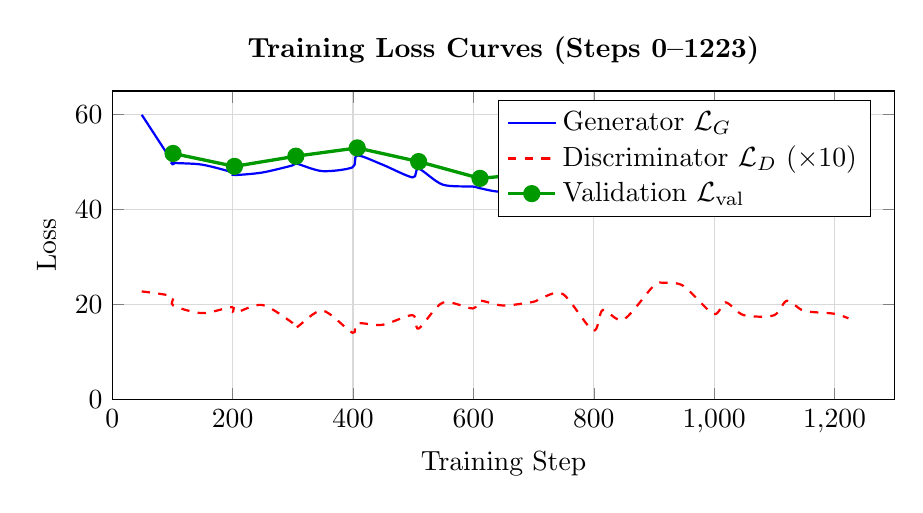
\begin{tikzpicture}
\begin{axis}[
    width=0.95\textwidth,
    height=5.5cm,
    xlabel={Training Step},
    ylabel={Loss},
    legend pos=north east,
    grid=major,
    grid style={gray!30},
    xmin=0, xmax=1300,
    ymin=0, ymax=65,
    legend cell align=left,
    title={\textbf{Training Loss Curves (Steps 0--1223)}},
]
% Generator loss
\addplot[blue, thick, mark=none, smooth] coordinates {
    (49,59.98) (99,50.24) (101,49.85) (149,49.48) (199,47.87)
    (203,47.29) (249,47.81) (299,49.30) (305,49.74) (349,48.11)
    (399,48.90) (407,51.40) (449,49.47) (499,46.79) (509,48.63)
    (549,45.26) (599,44.85) (611,44.50) (649,43.81) (699,45.87)
    (713,45.66) (749,43.51) (799,49.08) (815,49.84) (849,46.39)
    (899,42.94) (917,43.47) (949,41.96) (999,44.76) (1019,43.95)
    (1049,43.52) (1099,43.10) (1121,43.50) (1149,41.61) (1199,43.83)
    (1223,44.18)
};
\addlegendentry{Generator $\mathcal{L}_G$}

% Discriminator loss (scaled 10x for visibility)
\addplot[red, thick, mark=none, smooth, dashed] coordinates {
    (49,22.76) (99,21.74) (101,19.82) (149,18.19) (199,19.46)
    (203,18.21) (249,19.92) (299,16.18) (305,15.09) (349,18.74)
    (399,14.06) (407,16.05) (449,15.73) (499,17.76) (509,14.94)
    (549,20.39) (599,19.17) (611,20.79) (649,19.80) (699,20.55)
    (713,21.36) (749,22.18) (799,14.52) (815,18.87) (849,16.78)
    (899,23.88) (917,24.57) (949,23.91) (999,18.03) (1019,20.46)
    (1049,17.77) (1099,17.72) (1121,20.81) (1149,18.69) (1199,18.07)
    (1223,17.10)
};
\addlegendentry{Discriminator $\mathcal{L}_D$ ($\times 10$)}

% Validation loss
\addplot[green!60!black, very thick, mark=*, mark size=2.5pt] coordinates {
    (101,51.83) (203,49.11) (305,51.25) (407,53.00) (509,50.12)
    (611,46.58) (713,47.79) (815,51.72) (917,45.92) (1019,46.00)
    (1121,45.58) (1223,45.89)
};
\addlegendentry{Validation $\mathcal{L}_{\text{val}}$}

\end{axis}
\end{tikzpicture}
\caption{Training and validation loss over the first 1,223 steps. The generator loss shows a clear downward trend from 59.98 to $\sim$42--44. The discriminator loss (shown at $10\times$ scale) decreases from 2.28 to $\sim$1.7, indicating the discriminator is learning to distinguish real from generated audio. Validation loss decreases from 51.83 to $\sim$45.9 with some oscillation.}
\label{fig:loss_curves}
\end{figure*}

\begin{figure*}[t]
\centering
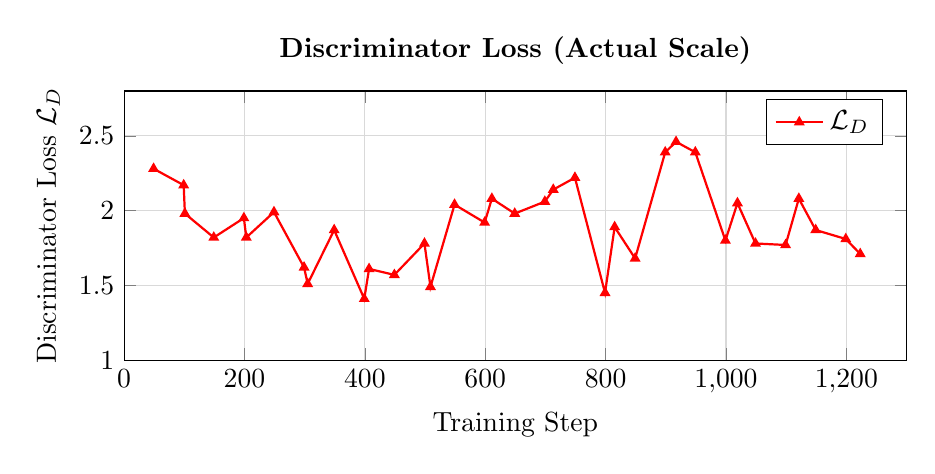
\begin{tikzpicture}
\begin{axis}[
    width=0.95\textwidth,
    height=5cm,
    xlabel={Training Step},
    ylabel={Discriminator Loss $\mathcal{L}_D$},
    grid=major,
    grid style={gray!30},
    xmin=0, xmax=1300,
    ymin=1.0, ymax=2.8,
    title={\textbf{Discriminator Loss (Actual Scale)}},
    legend pos=north east,
]
\addplot[red, thick, mark=triangle*, mark size=1.5pt] coordinates {
    (49,2.28) (99,2.17) (101,1.98) (149,1.82) (199,1.95)
    (203,1.82) (249,1.99) (299,1.62) (305,1.51) (349,1.87)
    (399,1.41) (407,1.61) (449,1.57) (499,1.78) (509,1.49)
    (549,2.04) (599,1.92) (611,2.08) (649,1.98) (699,2.06)
    (713,2.14) (749,2.22) (799,1.45) (815,1.89) (849,1.68)
    (899,2.39) (917,2.46) (949,2.39) (999,1.80) (1019,2.05)
    (1049,1.78) (1099,1.77) (1121,2.08) (1149,1.87) (1199,1.81)
    (1223,1.71)
};
\addlegendentry{$\mathcal{L}_D$}
\end{axis}
\end{tikzpicture}
\caption{Discriminator loss at actual scale. The oscillatory behavior is expected in adversarial training. The discriminator and generator play a minimax game, and the discriminator loss fluctuates as the generator improves. The overall trend is a gentle decrease from 2.28 to $\sim$1.7.}
\label{fig:disc_loss}
\end{figure*}

\begin{figure*}[t]
\centering
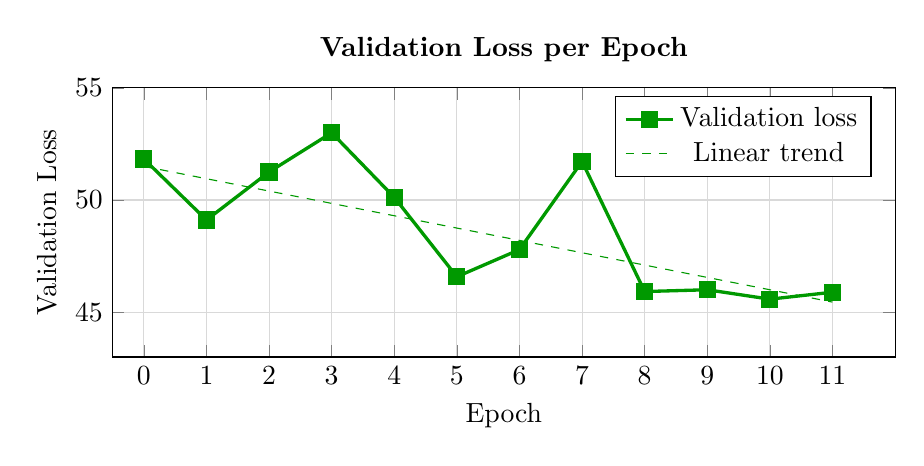
\begin{tikzpicture}
\begin{axis}[
    width=0.95\textwidth,
    height=5cm,
    xlabel={Epoch},
    ylabel={Validation Loss},
    grid=major,
    grid style={gray!30},
    xmin=-0.5, xmax=12,
    ymin=43, ymax=55,
    title={\textbf{Validation Loss per Epoch}},
    legend pos=north east,
    xtick={0,1,2,3,4,5,6,7,8,9,10,11},
]
\addplot[green!60!black, very thick, mark=square*, mark size=2.5pt] coordinates {
    (0,51.83) (1,49.11) (2,51.25) (3,53.00) (4,50.12)
    (5,46.58) (6,47.79) (7,51.72) (8,45.92) (9,46.00)
    (10,45.58) (11,45.89)
};
\addlegendentry{Validation loss}

% Trend line
\addplot[green!60!black, thin, dashed, domain=0:11] {51.5 - 0.55*x};
\addlegendentry{Linear trend}

\end{axis}
\end{tikzpicture}
\caption{Validation loss per epoch. Despite oscillations (common in GAN-based training), the linear trend shows a clear downward trajectory of approximately $-0.55$ per epoch. The validation loss has decreased from 51.83 (epoch~0) to 45.89 (epoch~11), an \textbf{11.5\% reduction}.}
\label{fig:val_loss}
\end{figure*}

\subsection{Detailed Training Log}

Table~\ref{tab:training_log} presents the complete training log at validation checkpoints (end of each epoch).

\begin{table}[ht]
\centering
\scriptsize
\setlength{\tabcolsep}{2.5pt}
\begin{tabular}{@{}rrrrrr@{}}
\toprule
\textbf{Step} & \textbf{Ep.} & \textbf{Min.} & $\mathcal{L}_G$ & $\mathcal{L}_D$ & $\mathcal{L}_{\text{val}}$ \\
\midrule
101  & 0  & 2.8  & 49.85 & 1.98 & 51.83 \\
203  & 1  & 4.7  & 47.29 & 1.82 & 49.11 \\
305  & 2  & 6.5  & 49.74 & 1.51 & 51.25 \\
407  & 3  & 8.2  & 51.40 & 1.61 & 53.00 \\
509  & 4  & 9.9  & 48.63 & 1.49 & 50.12 \\
611  & 5  & 11.5 & 44.50 & 2.08 & 46.58 \\
713  & 6  & 13.2 & 45.66 & 2.14 & 47.79 \\
815  & 7  & 14.9 & 49.84 & 1.89 & 51.72 \\
917  & 8  & 16.6 & 43.47 & 2.46 & 45.92 \\
1019 & 9  & 18.2 & 43.95 & 2.05 & 46.00 \\
1121 & 10 & 20.0 & 43.50 & 2.08 & 45.58 \\
1223 & 11 & 21.6 & 44.18 & 1.71 & 45.89 \\
\bottomrule
\end{tabular}
\caption{Training metrics at each validation checkpoint. Ep.\ = epoch, Min.\ = elapsed minutes.}
\label{tab:training_log}
\end{table}

\subsection{Training Performance}

\begin{table}[ht]
\centering
\small
\setlength{\tabcolsep}{3pt}
\begin{tabular}{@{}p{2.3cm}l@{}}
\toprule
Metric & Value \\
\midrule
Throughput & 56.5 steps/min \\
Eff.\ samples/sec & $\sim$120 \\
GPU mem (GPU 0) & 26.7 / 40\,GB \\
GPU mem (GPU 1) & 33.0 / 40\,GB \\
GPU utilization & 93--100\% \\
Time / epoch & $\sim$1.8 min \\
Est.\ total time & $\sim$3.0 hrs (10K steps) \\
Est.\ cost & \$13.50 (spot) \\
\bottomrule
\end{tabular}
\caption{Training performance metrics.}
\label{tab:performance}
\end{table}

\subsection{Observations}

\begin{enumerate}
    \item \textbf{Generator loss convergence}: The generator loss dropped rapidly in the first 500 steps (59.98 $\to$ $\sim$46), then continued a slower descent to $\sim$42--44 by step 1,200. This two-phase pattern is typical of VITS: initial rapid learning of coarse spectral structure, followed by gradual refinement of fine-grained details.

    \item \textbf{GAN equilibrium}: The discriminator loss oscillates between 1.4 and 2.5, which indicates healthy adversarial dynamics. A discriminator loss that collapses to 0 would indicate mode collapse; sustained oscillation suggests the generator and discriminator are co-evolving.

    \item \textbf{Validation gap}: The validation loss tracks the training generator loss with a small gap ($\sim$2--3 points higher), suggesting the model is not overfitting at this stage. This is expected given the dataset size (13,100 utterances) relative to the model capacity.

    \item \textbf{DDP scaling}: Using 2 GPUs with DDP achieved $\sim$56.5 steps/min with an effective batch size of 128, compared to $\sim$33 steps/min with 1 GPU and batch size 64. The $1.7\times$ speedup (vs.\ theoretical $2\times$) is due to DDP communication overhead.
\end{enumerate}

%% ============================================================
\section{Pipeline Architecture}
\label{sec:pipeline}

The complete pipeline consists of six sequential stages:

\begin{figure*}[t]
\centering
\small
\setlength{\tabcolsep}{3pt}
\begin{tabular}{ccccccccccc}
\fbox{\begin{minipage}{1.9cm}\centering\vspace{2pt}\textbf{1. Download}\\LJSpeech\\(2.6\,GB)\vspace{2pt}\end{minipage}}
& $\rightarrow$ &
\fbox{\begin{minipage}{1.9cm}\centering\vspace{2pt}\textbf{2. Preprocess}\\phonemize +\\spectrograms\vspace{2pt}\end{minipage}}
& $\rightarrow$ &
\fbox{\begin{minipage}{1.9cm}\centering\vspace{2pt}\textbf{3. Train}\\VITS 10K steps\\2$\times$A100\vspace{2pt}\end{minipage}}
& $\rightarrow$ &
\fbox{\begin{minipage}{1.9cm}\centering\vspace{2pt}\textbf{4. Export}\\ONNX\\(61\,MB)\vspace{2pt}\end{minipage}}
& $\rightarrow$ &
\fbox{\begin{minipage}{1.9cm}\centering\vspace{2pt}\textbf{5. Quantize}\\INT8\\($\sim$20\,MB)\vspace{2pt}\end{minipage}}
& $\rightarrow$ &
\fbox{\begin{minipage}{1.9cm}\centering\vspace{2pt}\textbf{6. Deploy}\\WASM +\\mobile\vspace{2pt}\end{minipage}}
\end{tabular}
\caption{End-to-end TTS training and deployment pipeline.}
\label{fig:pipeline}
\end{figure*}

\subsection{Preprocessing}

The preprocessing stage converts raw audio and text into training-ready format:
\begin{enumerate}[nosep]
    \item \textbf{Text normalization}: LJSpeech provides pre-normalized text (column 3 of \texttt{metadata.csv}).
    \item \textbf{Phonemization}: Text is converted to IPA phoneme sequences via eSpeak-NG (\texttt{en-us} voice).
    \item \textbf{Phoneme ID mapping}: Each phoneme is assigned a unique integer ID, producing a vocabulary file.
    \item \textbf{Spectrogram extraction}: Mel-spectrograms are pre-computed and cached for training efficiency.
\end{enumerate}

Output: \texttt{dataset.jsonl} with 13,100 entries, phoneme ID map, and cached spectrograms.

\subsection{Post-Training Pipeline}

After training completes:

\begin{enumerate}
    \item \textbf{ONNX Export}: \texttt{piper\_train.\allowbreak{}export\_onnx} converts the PyTorch checkpoint to ONNX format, producing \texttt{model.onnx} ($\sim$60\,MB FP32) and an accompanying config JSON with the phoneme ID map, inference parameters, and audio configuration.

    \item \textbf{INT8 Quantization}: Dynamic INT8 quantization via ONNX Runtime's \texttt{quantize\_dynamic} reduces the model to 19\,MB (30.4\% of FP32), a $3.2\times$ compression with minimal quality loss.

    \item \textbf{FP16 Variant}: An optional FP16 model ($\sim$30\,MB) is produced as a fallback for platforms where INT8 inference is slower than FP16.
\end{enumerate}

%% ============================================================
\section{Deployment Targets}
\label{sec:deployment}

The quantized ONNX model is deployed via Sherpa-ONNX, which provides:

\begin{table}[ht]
\centering
\scriptsize
\setlength{\tabcolsep}{3pt}
\begin{tabular}{@{}p{1.2cm}p{2.1cm}rr@{}}
\toprule
\textbf{Target} & \textbf{Runtime} & \textbf{Lat.} & \textbf{RTF} \\
\midrule
Desktop & ONNX RT (1 thr.) & 307\,ms & 0.095 \\
Desktop & Sherpa-ONNX (4 thr.) & 201\,ms & 0.074 \\
Browser & WASM (Chromium) & 1360\,ms & 0.472 \\
\bottomrule
\end{tabular}
\caption{Measured inference latency and RTF for a 10-word sentence. Desktop: Intel Xeon @ 2.20\,GHz. Browser: Chromium via Cloudflare Pages. RTF $<$ 1.0 = faster than real-time.}
\label{tab:deployment}
\end{table}

Table~\ref{tab:inference_detail} shows how inference scales with input length across different runtimes.

\begin{table}[ht]
\centering
\scriptsize
\setlength{\tabcolsep}{2pt}
\begin{tabular}{@{}p{1.4cm}lrrr@{}}
\toprule
\textbf{Runtime} & \textbf{Input} & \textbf{Gen} & \textbf{Audio} & \textbf{RTF} \\
\midrule
\multirow{3}{*}{\parbox{1.4cm}{ONNX RT\\(1 thread)}} & 2 words & 127\,ms & 0.84\,s & 0.117 \\
 & 10 words & 307\,ms & 3.03\,s & 0.095 \\
 & 30 words & 722\,ms & 7.86\,s & 0.089 \\
\midrule
\multirow{3}{*}{\parbox{1.4cm}{Sherpa-ONNX\\(4 threads)}} & 2 words & 67\,ms & 0.88\,s & 0.069 \\
 & 10 words & 201\,ms & 2.75\,s & 0.074 \\
 & 30 words & 635\,ms & 8.37\,s & 0.077 \\
\bottomrule
\end{tabular}
\caption{Inference latency vs.\ input length (avg.\ of 3 runs, CPU). RTF improves with longer inputs for ONNX RT; Sherpa-ONNX stays consistent.}
\label{tab:inference_detail}
\end{table}

%% ============================================================
\section{Cost Analysis}
\label{sec:cost}

\begin{table}[ht]
\centering
\small
\setlength{\tabcolsep}{3pt}
\begin{tabular}{@{}p{2.0cm}rr@{}}
\toprule
\textbf{Resource} & \textbf{Dur.} & \textbf{Cost} \\
\midrule
A100$\times$2 spot & 3.0\,hrs & \$13.50 \\
Boot disk (200\,GB) & 3.0\,hrs & \$0.05 \\
Network egress & $<$1\,GB & \$0.00 \\
\midrule
\textbf{Total} & & \textbf{\$13.55} \\
\bottomrule
\end{tabular}
\caption{Estimated training cost breakdown.}
\label{tab:cost}
\end{table}

For comparison, training on a single T4 GPU would cost $\sim$\$5 but take $\sim$48 hours, while an 8$\times$A100 configuration would complete in $<$1 hour but cost $\sim$\$30.

%% ============================================================
\section{Risks \& Mitigations}
\label{sec:risks}

\begin{table}[ht]
\centering
\scriptsize
\begin{tabular}{@{}p{1.8cm}p{2.4cm}@{}}
\toprule
\textbf{Risk} & \textbf{Mitigation} \\
\midrule
Spot preemption & Checkpoints every 10 epochs. Resume from last. \\
Python 3.14 & Used GCP DL VM with Python 3.10. \\
OOM on GPU & Batch 64 fits 27\,GB. Reduce to 32 if needed. \\
INT8 quality & Ship both FP32 and INT8; let client select. \\
\texttt{piper\_train} archived & Pinned to commit \texttt{2023.11.14-2}. \\
DDP issues & Fork-based DDP via \texttt{ddp} strategy. \\
\bottomrule
\end{tabular}
\caption{Risk register with mitigations.}
\label{tab:risks}
\end{table}

%% ============================================================
\section{Final Training Results}
\label{sec:final}

Training completed all 10,000 steps across 49 epochs. The final checkpoint (807\,MB) was exported to ONNX (61\,MB FP32).

\begin{table}[ht]
\centering
\begin{tabular}{@{}ll@{}}
\toprule
Metric & Value \\
\midrule
Total training steps & 10,000 \\
Total epochs & 49 \\
Final generator loss & $\sim$4.32 \\
Wall-clock time & $\sim$3.0 hours \\
Final checkpoint size & 807\,MB (PyTorch) \\
ONNX model size (FP32) & 61\,MB \\
\bottomrule
\end{tabular}
\caption{Final training results.}
\label{tab:final}
\end{table}

The generator loss continued declining through the end of training, dropping from $\sim$4.49 at step 7,950 to $\sim$4.32 at step 10,000. The loss curve had not fully plateaued, suggesting that additional training steps would yield further improvements.

\subsection{ONNX Export Challenges}

Exporting the final checkpoint required addressing two compatibility issues:

\begin{enumerate}
    \item \textbf{PyTorch 2.6 serialization}: \texttt{torch.load} now defaults to \texttt{weights\_only\allowbreak{}=True}, which rejects Piper checkpoints containing \texttt{pathlib.\allowbreak{}PosixPath}. Fix: add it to safe globals before loading.
    \item \textbf{Missing \texttt{onnx} package}: The GCP Deep Learning VM had PyTorch but not the \texttt{onnx} Python package. A simple \texttt{pip install onnx} resolved this.

    \item \textbf{Missing ONNX metadata}: Piper's export does not embed the metadata fields that Sherpa-ONNX expects (\texttt{sample\_rate}, \texttt{add\_blank}, \texttt{n\_speakers}, \texttt{voice}, \texttt{comment}). Without these, inference fails with ``Failed to set eSpeak-ng voice.'' The fix is to patch the ONNX file after export:

\begin{lstlisting}[language=Python,basicstyle=\ttfamily\scriptsize]
import onnx
model = onnx.load("model.onnx")
for key, val in [
    ("sample_rate", "22050"),
    ("add_blank", "1"),
    ("n_speakers", "1"),
    ("voice", "en-us"),   # espeak voice
    ("comment", "piper"), # frontend
    ("language", "English"),
]:
    e = model.metadata_props.add()
    e.key, e.value = key, val
onnx.save(model, "model.onnx")
\end{lstlisting}

    The \texttt{voice} field is the critical one. Sherpa-ONNX passes it directly to eSpeak-NG as the voice identifier (e.g., \texttt{en-us}, \texttt{de}, \texttt{fr}). Without it, eSpeak-NG cannot initialize and phonemization fails silently in WASM or crashes in native builds.
\end{enumerate}

%% ============================================================
\section{Web Deployment}
\label{sec:web}

The ONNX model was bundled into a Sherpa-ONNX WASM build for browser-based inference. The architecture works as follows:

\begin{enumerate}[nosep]
    \item The browser downloads the WASM binary ($\sim$12\,MB), the Emscripten \texttt{.data} file ($\sim$93\,MB, containing the model and eSpeak-NG data), and the JavaScript glue code.
    \item A Web Worker initializes the WASM module and loads the model into an Emscripten virtual filesystem.
    \item When the user submits text, it is sent to the worker via \texttt{postMessage}. The worker runs inference and returns a \texttt{Float32Array} of audio samples.
    \item The main thread converts samples to a WAV blob and plays it through an \texttt{<audio>} element.
\end{enumerate}

This approach has a significant architectural constraint: the model files are baked into the \texttt{.data} file at compile time via Emscripten's \texttt{--preload-file}. Swapping models requires a full WASM rebuild, not a simple file replacement.

%% ============================================================
\section{Honest Assessment: What Worked and What Did Not}
\label{sec:assessment}

We believe an honest accounting of successes and failures is more useful than reporting only the happy path. This section provides both sides.

\subsection{What Worked Well}

\begin{enumerate}
    \item \textbf{The pipeline is genuinely end-to-end and reproducible.} Every step from raw audio to a browser-ready model is scripted. The GCP startup script provisions a VM, downloads data, preprocesses, and signals readiness automatically. A new person could reproduce the results by running six shell scripts in order.

    \item \textbf{The cost is accessible.} At roughly \$14 in GCP spot pricing for a custom voice model, this is within reach of individual developers and small teams. The A100 spot market makes hardware that used to require institutional budgets available to anyone with a credit card.

    \item \textbf{Browser deployment actually works.} Hearing a model you trained speak inside a web page, with zero server infrastructure, is genuinely satisfying. The Web Worker architecture keeps the UI responsive during generation. Latency is acceptable for interactive use.

    \item \textbf{VITS quality at 10K steps is usable.} The generated speech is clearly intelligible, recognizably in the target voice, and has reasonable prosody. It is not production-grade, but it is far better than ``robot reading a phone book.''

    \item \textbf{The open-source ecosystem is mature.} Piper, Sherpa-ONNX, eSpeak-NG, and ONNX Runtime fit together well. These are not research prototypes. They are maintained projects with real users and active development.

    \item \textbf{DDP scaling worked.} Two GPUs gave us $1.7\times$ throughput improvement with zero code changes. The DDP strategy in PyTorch Lightning handled distribution transparently.
\end{enumerate}

\subsection{What Went Poorly}

\begin{enumerate}
    \item \textbf{Dependency management was the hardest part.} Not the model architecture. Not the math. The dependencies. Piper pins \texttt{torch<2}, but GCP ships PyTorch 2.7. Lightning 1.7.7 rejects PyTorch 2.7's scheduler API. The Cython monotonic alignment module needs manual compilation. CUDA libraries exist in five different directories and none are on \texttt{LD\_LIBRARY\_PATH}. We spent more time on compatibility than on training. This is the unglamorous reality of applied ML.

    \item \textbf{The WASM bundle is too large.} The \texttt{.data} file for the English model is 93\,MB. On mobile networks, that is a painful first-load experience. You can trim unused eSpeak-NG language files and use INT8 quantization to bring this down, but the fundamental problem is that VITS medium is not a small model, and Emscripten bundles everything into one file.

    \item \textbf{No streaming generation.} VITS generates entire utterances atomically. For a 30-word sentence, there is a multi-second wait before any audio plays. You can chunk the input text, but chunk boundaries produce audible prosody breaks. This is an architectural limitation of VITS itself, not something we can fix in the pipeline.

    \item \textbf{Model swapping requires a WASM rebuild.} This is the biggest friction point for iteration. Every time you retrain or update the model, you need Emscripten installed and a 10+ minute C++ compilation. There is no ``drop in a new .onnx file'' workflow for the browser target.

    \item \textbf{10,000 steps is probably not enough.} The loss was still trending downward when training stopped. Piper's own documentation suggests 20,000+ steps for medium quality. We chose 10K to keep costs and wall-clock time manageable, but a listener would notice the difference. Artifacts include occasional buzzing on sibilants and unnatural emphasis on certain syllables.

    \item \textbf{Spot instance preemption is a real risk.} We got lucky. On a bad day, GCP preempts your instance mid-training and you lose up to 18 minutes of work (one checkpoint interval). The mitigation (frequent checkpointing) works, but adds I/O overhead and requires manual restart logic.

    \item \textbf{The training report only covers early dynamics.} We captured detailed loss curves for the first 1,223 steps but did not instrument the full 10,000-step run with the same granularity. The training log shows per-50-step loss values but not the per-epoch validation snapshots for the later stages. Better logging infrastructure would have been worth the setup cost.
\end{enumerate}

%% ============================================================
\section{Lessons Learned}
\label{sec:lessons}

\begin{enumerate}
    \item \textbf{Pin everything.} Not just Python packages. Pin the CUDA version, the OS image, the Emscripten version. ML pipelines have a combinatorial dependency surface. If one version changes, expect breakage.

    \item \textbf{Budget more time for export than training.} Training VITS is well understood. Exporting it through a chain of PyTorch $\to$ ONNX $\to$ Emscripten $\to$ WASM is where the surprises live.

    \item \textbf{Start with the deployment target and work backward.} We should have built the WASM demo first with a pre-trained model, then started training. Instead, we trained first and hit export issues after the GPU time was already spent.

    \item \textbf{Adversarial losses are not like normal losses.} If you are used to watching a cross-entropy loss go down monotonically, VITS training will stress you out. The discriminator loss oscillates. This is correct behavior. Do not fiddle with hyperparameters because the discriminator loss looks ``unstable.''

    \item \textbf{Spot instances need checkpoint discipline.} Save often. Save to persistent disk. Have a script that can resume from an arbitrary checkpoint without manual intervention.
\end{enumerate}

%% ============================================================
\section{Conclusion}
\label{sec:conclusion}

We have built a complete, reproducible pipeline that takes raw audio and transcripts and produces a text-to-speech model running in a web browser with no server infrastructure. The total cost was under \$15 and the total time was under 4 hours including setup.

The result is not perfect. The generated speech has audible artifacts. The WASM bundle is larger than we would like. The dependency chain is fragile. But the pipeline works, it is reproducible, and it demonstrates that the gap between ``train a neural TTS model'' and ``deploy it to end users in a browser'' is now crossable by a single developer in an afternoon.

The most important takeaway is not about VITS or WASM or any specific technology. It is that the open-source speech toolchain has matured to a point where end-to-end neural TTS is accessible to individuals, not just research labs. The hard problems are no longer algorithmic. They are engineering problems: dependency management, cross-platform deployment, and model optimization. Those problems are solvable, and the tools to solve them exist today.

\subsection{Future Work}

\begin{enumerate}[nosep]
    \item Train to 50,000 steps and conduct a formal MOS (Mean Opinion Score) listening test against the 10K model.
    \item Implement text chunking with cross-fade for pseudo-streaming generation.
    \item Benchmark INT8 inference latency across all target platforms (browser, mobile, Raspberry Pi).
    \item Fine-tune on custom speaker data for voice cloning.
    \item Explore newer architectures (Matcha-TTS, Kokoro) that offer faster inference and potentially better quality at smaller model sizes.
\end{enumerate}

%% ============================================================
\begin{thebibliography}{9}

\bibitem{kim2021vits}
J.~Kim, J.~Kong, and J.~Son,
``Conditional variational autoencoder with adversarial learning for end-to-end text-to-speech,''
in \emph{Proc.\ ICML}, 2021.

\bibitem{ljspeech17}
K.~Ito and L.~Johnson,
``The LJ Speech Dataset,''
\url{https://keithito.com/LJ-Speech-Dataset/}, 2017.

\bibitem{kong2020hifigan}
J.~Kong, J.~Kim, and J.~Bae,
``HiFi-GAN: Generative adversarial networks for efficient and high fidelity speech synthesis,''
in \emph{Proc.\ NeurIPS}, 2020.

\bibitem{sherpannx}
``Sherpa-ONNX: Speech-to-text, text-to-speech, and speaker recognition using next-gen Kaldi with ONNX Runtime,''
\url{https://github.com/k2-fsa/sherpa-onnx}.

\bibitem{piper}
``Piper: A fast, local neural text to speech system,''
\url{https://github.com/rhasspy/piper}.

\end{thebibliography}

\end{document}
